\documentclass[a4paper, 10pt, DIV=16, parskip = full, twocolumn = true]{scrartcl}
\usepackage{setspace}
\usepackage{amsmath}
\usepackage{amssymb}
\usepackage{lastpage}
\usepackage{scrlayer-scrpage}
\usepackage[utf8]{inputenc}
\usepackage{graphicx}
%\usepackage{subcaption}
\usepackage[section]{placeins}
%\usepackage{pdfpages}
%\usepackage{layout}
\usepackage{enumitem}
\usepackage{booktabs}

\usepackage{placeins}
\usepackage{inconsolata}
\usepackage[bottom]{footmisc}
\usepackage[group-digits=false]{siunitx}
\usepackage{caption}

%\usepackage{lipsum}
\usepackage{cuted}

%\setlength{\parskip}{3pt}
\setlength{\columnsep}{15pt}
%\onehalfspacing
%\setlength{\columnseprule}{0.1pt}
\cofoot{\thepage\ of \pageref{LastPage}}
\subject{METU ME462 Mechatronic Design, Spring 2020}
\title{Design Evaluation: Design and manufacture of a wheeled robot controlled by the movement of a fish swimming inside an aquarium}
\author{\textbf{Say My Name} \\ Sercan Aslan / 1909902 \\ Ali Levent Çınar / 2234532 \\ Yusuf Can Coşkun / 1939420}
\date{March 2, 2020}

\renewcommand{\familydefault}{\sfdefault}
\renewcommand*\thesection{\arabic{section}.}
%\renewcommand*\thesubsection{\!\!\!}
\renewcommand{\theequation}{\arabic{equation}}
\renewcommand{\thefigure}{\arabic{figure}}
\renewcommand{\thetable}{\arabic{table}}

% squeeze tables
\renewcommand{\arraystretch}{0.7}
\renewcommand{\tabcolsep}{1mm}

\begin{document}
	\maketitle
	\thispagestyle{scrheadings}
	%\includepdf[pages=-]{Images/Title-Page.pdf} % set twocolumn = false
	\pagenumbering{arabic}

%%%%%%%%%%%%%%%%%%%%%%%%%%%%%%%%%%%%%%%%%%%%%%%%%%%%%%%%%%%%%%%%%%%%%%%%%%%%%%%%%%%%%%%%%%%%%%%%%%%%%%%%%%%	
%\section{Introduction}

Design alternatives has been explored for each function of a wheeled robot controlled by the movement of a fish swimming inside an aquarium (Robofish). The functional decomposition schematic of Robofish is as shown in Figure \ref{fig:funcdecomp}. The generated concepts for each function and their respective evaluation criteria has been summarized in Table \ref{table:concepts} and \ref{table:criterion}. Note that the functions, concepts and evaluation criteria will be referred by their function ID (FID), concept ID (CID) and evaluation ID (EID), respectively, in the remainder of this document. The CID of the highest scoring concepts will be presented in bold throughout the document. Datum concepts will be denoted with a star. The evaluation criteria are weighted using the analytic hierarchy process (AHP) in Tables \ref{table:AHP1-1}-\ref{table:AHP5-2}. The generated concepts are systematically evaluated in Tables \ref{table:pugh1-1}-\ref{table:pugh5-2} using weighted decision-matrix (Pugh) method.

\begin{strip}
	\break\break\break
	\centering
	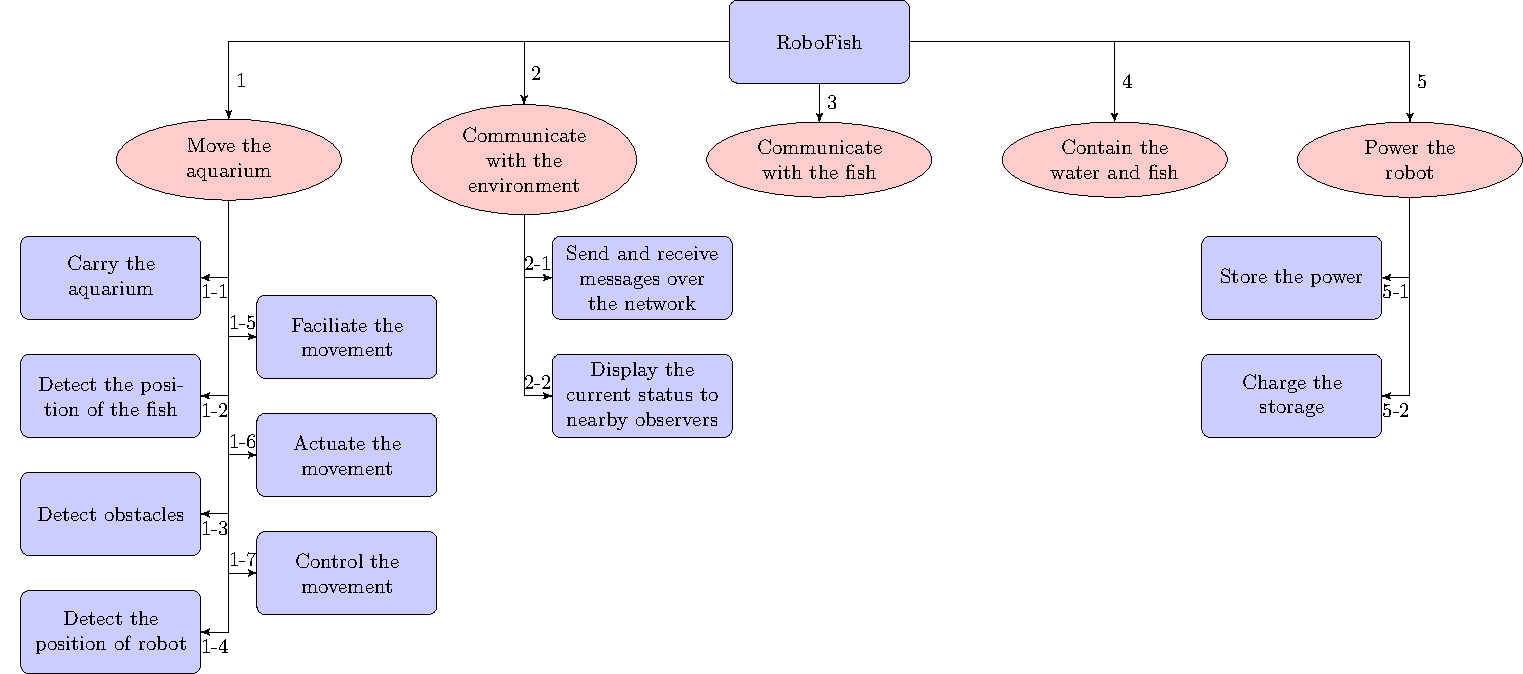
\includegraphics[width=0.8\pagewidth]{../functional_decomposition/functional_decomposition.pdf}
	\captionof{figure}{The functional decomposition.}
	\label{fig:funcdecomp}
\end{strip}

%%%%%%%%%%%%%%%%%%%%%%%%%%%%%%%%%%%%%%%%%%%%%%%%%%%%%%%%%%%%%%%%%%%%%%%%%%%%%%%%%%%%%%%%%%%%%%%%

\begin{table*}
\centering
\caption{Generated concepts for the functions of Robofish}
	\begin{tabular}{rlrl}
	\toprule
		FID & Function Name & CID & Concept \\
	\midrule
		1-1 & Carry the aquarium & 1-1C1 & Glued platform \\	
	 	& & \textbf{1-1C2} & Positive contact due to gravity \\	
		& & 1-1C3 & Assembled to a platform with holes \\	
		& & 1-1C4 & Components directly assembled \\	
		& & 1-1C5 & Components directly assembled, segmented aquarium \\	
		1-2 & Detect the position of fish & \textbf{1-2C1} & Webcam \& Raspberry Pi \\
		& & 1-2C2 & ESP32-CAM \\	
		& & 1-2C3 & Raspberry Pi Camera \\	
		1-3 & Detect the obstacles & 1-3C1 & Ultrasonic sensors \\
		& & 1-3C2 & Wide lens camera on the robot \\	
		& & 1-3C3 & Overhead camera (not attached to the robot) \\
		1-4 & Detect the position of robot & 1-4C1 & Overhead camera (not attached to the robot) \\	 
		& & \textbf{1-4C2} & Wide lens camera on the robot \\
		& & 1-4C3 & No camera (using available sensor data \& encoder) \\
		1-5 & Facilitate the movement & \textbf{1-5C1} & 3D printed mechanum wheels \\
		& & 1-5C2 & Machined mechanum wheels \\	
		& & 1-5C3 & Differential drive \\
		& & 1-5C4 & Tracks \\	
		& & 1-5C5 & Steered wheels \\
		1-6 & Actuate the movement & \textbf{1-6C1} & Brushless DC motor \\
		& & 1-6C2 & Brushed DC motor \\	
		& & 1-6C3 & Stepper motor \\
		1-7 & Control the movement & \textbf{1-7C1} & Raspberry Pi \\
		& & 1-7C2 & Dedicated PC (connected via cable or network module) \\	
		& & 1-7C3 & Arduino microprocessor \\	
		2-1 & Send \& receive network messages & \textbf{2-1C1} & Raspberry Pi \\
		& & 2-1C2 & Network module \\	
		& & 2-1C3 & Arduino Wi-Fi module \\
		2-2 & Display the current status & \textbf{2-2C1} & LED indicator lights\\
		& & 2-2C2 & Speakers \\	
		& & 2-2C3 & Monitor \\	
		3-1 & Communicate with the fish & \textbf{3-1C1} & LED lighting \\
		& & 3-1C2 & Monitor (attached to the robot) \\		
		4-1 & Contain the water \& fish & \textbf{4-1C1} & Plastic aquarium \\
		& & 4-1C2 & Spherical glass aquarium \\	
		& & 4-1C3 & Prismatic glass aquarium \\
		5-1 & Store the power & 5-1C1 & Ni-Cad battery \\
		& & 5-1C2 & Li-Po battery \\	
		& & 5-1C3 & Li-Ion battery \\
		& & \textbf{5-1C4} & Dry accumulator \\	
		5-2 & Charge the storage & \textbf{5-2C1} & Dangling magnet attached to the room \\
		& & \textbf{5-2C2} & Dangling magnet attached to the robot \\	
		& & 5-2C3 & Mechanical connection \\
		& & 5-2C4 & Inductive charging \\
	\bottomrule
	\end{tabular}
\label{table:concepts}
\end{table*}

\begin{table*}
	\centering
	\caption{Concept evaluation criteria for the functions of Robofish}
	\begin{tabular}{rlrl}
		\toprule
		FID & Function Name & EID & Evaluation Criterion \\
		\midrule
		1-1 & Carry the aquarium & 1-1E1 & Cost\\	
		& & 1-1E2 & Removability (important for cleaning, removing water)\\	
		& & 1-1E3 & Durability \\	
		& & 1-1E4 & Aesthetics \\	
		& & 1-1E5 & Manufacturability \\	
		1-2 & Detect the position of the fish & 1-2E1 & Resolution \\
		& & 1-2E2 & Response time \\	
		& & 1-2E3 & Cost \\	
		& & 1-2E4 & Mountability \\	
		& & 1-2E5 & Upgradability \\	
		1-3 & Detect the obstacles & 1-3E1 & Precision \\
		& & 1-3E2 & Cost \\	
		& & 1-3E3 & Response time \\
		& & 1-3E4 & Manufacturability \\
		1-4 & Detect the position of the robot & 1-4E1 & Cost \\
		& & 1-4E2 & Response time \\	
		& & 1-4E3 & Precision \\
		& & 1-4E4 & Manufacturability \\
		1-5 & Facilitate the movement & 1-5E1 & Smoothness \\
		& & 1-5E2 & Range of motion \\	
		& & 1-5E3 & Cost  \\
		& & 1-5E4 & Durability (includes weight carrying capacity) \\	
		& & 1-5E5 & Manufacturability \\
		1-6 & Actuate the movement & 1-6E1 & Noise \\
		& & 1-6E2 & Precision \\	
		& & 1-6E3 & Durability \\
		& & 1-6E4 & Cost \\
		& & 1-6E5 & Ease of control (in order to ensure smooth motion) \\
		1-7 & Control the movement & 1-7E1 & Cost \\
		& & 1-7E2 & Performance \\	
		& & 1-7E3 & Upgradability \\
		& & 1-7E4 & Continuity (resistance against power loss) \\	
		2-1 & Send \& receive network messages & 2-1E1 & Cost \\
		& & 2-1E2 & Performance \\	
		& & 2-1E3 & Upgradability \\
		2-2 & Display the current status & 2-2E1 & Cost\\
		& & 2-2E2 & Manufacturability \\	
		& & 2-2E3 & Aesthetics \\	
		& & 2-2E4 & Range of messages (ability to convey different messages) \\	
		& & 2-2E5 & Power consumption \\	
		3-1 & Communicate with the fish & 3-1E1 & Cost \\
		& & 3-1E2 & Manufacturability \\		
		& & 3-1E3 & Range of messages (ability to convey different messages) \\	
		& & 3-1E4 & Power consumption \\	
		4-1 & Contain the water \& fish & 4-1E1 & Cost \\
		& & 4-1E2 & Mountability \\	
		& & 4-1E3 & Weight \\
		& & 4-1E4 & Visibility (by the camera, if one exists) \\
		& & 4-1E5 & Aesthetics \\
		5-1 & Store the power & 5-1E1 & Cost \\
		& & 5-1E2 & Durability (life of the battery) \\	
		& & 5-1E3 & Capacity per weight \\
		5-2 & Charge the storage & 5-2E1 & Cost \\
		& & 5-2E2 & Manufacturability \\	
		& & 5-2E3 & Charging time (better if less)\\
		& & 5-2E4 & Durability \\
		\bottomrule
	\end{tabular}
\label{table:criterion}
\end{table*}

%%%%%%%%%%%%%%%%%%%%%%%%%%%%%%%%%%%%%%%%%%%%%%%%%%%%%%%%%%%%%%%%%%%%%%%%%%%%%%%%%%%%%%%%%%%%%%%%

%\section{Criteria weighting}

\begin{table}
	\centering
	\caption{AHP for 1-1: Carry the aquarium}
	\begin{tabular}{l|sssssS}
		\toprule
		& \text{1-1E1} & \text{1-1E2} & \text{1-1E3} & \text{1-1E4} & \text{1-1E5} & \text{Weight (\%)} \\
		\midrule
		1-1E1 & 1 & 1/5 & 1/7 & 1/3 & 5 & 12.4 \\
		1-1E2 & & 1 & 3 & 7 & 5 & 43.3 \\
		1-1E3 & & & 1 & 7 & 1 & 24.5 \\
		1-1E4 & & & & 1 & 1/5 & 7.08 \\
		1-1E5 & & & & & 1 & 12.7 \\
	\bottomrule
	\end{tabular}
	\label{table:AHP1-1}
	
	\centering
	\caption{AHP for 1-2: Detect the position of fish}
	\begin{tabular}{l|sssssS}
		\toprule
		& \text{1-2E1} & \text{1-2E2} & \text{1-2E3} & \text{1-2E4} & \text{1-2E5} & \text{Weight (\%)} \\
		\midrule
		1-2E1 & 1 & 1 & 7 & 3 & 3 & 34.5\\
		1-2E2 & & 1 & 5 & 3 & 5 & 35.6 \\
		1-2E3 & & & 1 & 1/3 & 1/3 & 4.94 \\
		1-2E4 & & & & 1 & 3 & 15.4 \\
		1-2E5 & & & & & 1 & 9.49 \\
		\bottomrule
	\end{tabular}
	\label{table:AHP1-2}
	
	\centering
	\caption{AHP for 1-3: Detect the obstacles}
	\begin{tabular}{l|ssssS}
		\toprule
		& \text{1-3E1} & \text{1-3E2} & \text{1-3E3} & \text{1-3E4} & \text{Weight (\%)} \\
		\midrule
		1-3E1 & 1 & 5 & 1 & 3 & 37.2 \\
		1-3E2 & & 1 & 1/5 & 1/3 & 6.74 \\
		1-3E3 & & & 1 & 5 & 42.6 \\
		1-3E4 & & & & 1 & 13.4 \\
		\bottomrule
	\end{tabular}
	\label{table:AHP1-3}
	
	\centering
	\caption{AHP for 1-4: Detect the position of the robot}
	\begin{tabular}{l|ssssS}
		\toprule
		& \text{1-4E1} & \text{1-4E2} & \text{1-4E3} & \text{1-4E4} & \text{Weight (\%)} \\
		\midrule
		1-4E1 & 1 & 1/5 & 1/5 & 1/3 & 6.87 \\
		1-4E2 & & 1 & 1 & 3 & 38.9 \\
		1-4E3 & & & 1 & 3 & 38.9 \\
		1-4E4 & & & & 1 & 15.3 \\
		\bottomrule
	\end{tabular}
	\label{table:AHP1-4}
	
	\centering
	\caption{AHP for 1-5: Facilitate the movement}
	\begin{tabular}{l|sssssS}
		\toprule
		& \text{1-5E1} & \text{1-5E2} & \text{1-5E3} & \text{1-5E4} & \text{1-5E5} & \text{Weight (\%)} \\
		\midrule
		1-5E1 & 1 & 3 & 7 & 5 & 3 & 45.8 \\
		1-5E2 & & 1 & 5 & 3 & 3 & 24.7 \\
		1-5E3 & & & 1 & 1/3 & 1/3 & 4.63 \\
		1-5E4 & & & & 1 & 3 & 14.4 \\
		1-5E5 & & & & & 1 & 10.5 \\
		\bottomrule
	\end{tabular}
	\label{table:AHP1-5}
	
	\centering
	\caption{AHP for 1-6: Actuate the movement}
	\begin{tabular}{l|sssssS}
		\toprule
		& \text{1-6E1} & \text{1-6E2} & \text{1-6E3} & \text{1-6E4} & \text{1-6E5} & \text{Weight (\%)} \\
		\midrule
		1-6E1 & 1 & 1/5 & 1/3 & 3 & 1/5 & 9.76 \\
		1-6E2 & & 1 & 1 & 5 & 3 & 34.1 \\
		1-6E3 & & & 1 & 5 & 3 & 31.3 \\
		1-6E4 & & & & 1 & 3 & 10.6 \\
		1-6E5 & & & & & 1 & 14.2 \\
		\bottomrule
	\end{tabular}
	\label{table:AHP1-6}

\end{table}

\begin{table}
	
	\centering
	\caption{AHP for 1-7: Control the movement}
	\begin{tabular}{l|ssssS}
		\toprule
		& \text{1-7E1} & \text{1-7E2} & \text{1-7E3} & \text{1-7E4} & \text{Weight (\%)} \\
		\midrule
		1-7E1 & 1 & 1/5 & 1/3 & 1/5 & 6.70 \\
		1-7E2 & & 1 & 3 & 3 & 49.1 \\
		1-7E3 & & & 1 & 1/3 & 15.1 \\
		1-7E4 & & & & 1  & 29.1 \\
		\bottomrule
	\end{tabular}
	\label{table:AHP1-7}
	
	\centering
	\caption{AHP for 2-1: Send \& receive network messages}
	\begin{tabular}{l|sssS}
		\toprule
		& \text{2-1E1} & \text{2-1E2} & \text{2-1E3} & \text{Weight (\%)} \\
		\midrule
		2-1E1 & 1 & 1/5 & 1/5 & 8.97 \\
		2-1E2 & & 1 & 3 & 60.7 \\
		2-1E3 & & & 1 & 30.3 \\
		\bottomrule
	\end{tabular}
	\label{table:AHP2-1}
	
	\centering
	\caption{AHP for 2-2: Display the current status}
	\begin{tabular}{l|sssssS}
		\toprule
		& \text{2-2E1} & \text{2-2E2} & \text{2-2E3} & \text{2-2E4} & \text{2-2E5} & \text{Weight (\%)} \\
		\midrule
		2-2E1 & 1 & 1/3 & 1/3 & 1/3 & 1/5 & 5.91 \\
		2-2E2 & & 1 & 1/5 & 1/3 & 1/3 & 10.5 \\
		2-2E3 & & & 1 & 1/3 & 1/3 & 19.1 \\
		2-2E4 & & & & 1 & 1/3 & 23.9 \\
		2-2E5 & & & & & 1 & 40.6 \\
		\bottomrule
	\end{tabular}
	\label{table:AHP2-2}
	
    \centering
	\caption{AHP for 3-1: Communicate with the fish}
	\begin{tabular}{l|ssssS}
		\toprule
		& \text{3-1E1} & \text{3-1E2} & \text{3-1E3} & \text{3-1E4} & \text{Weight (\%)} \\
		\midrule
		3-1E1 & 1 & 1/3 & 1/3 & 1/5 & 7.68 \\
		3-1E2 & & 1 & 1/3 & 1/3 & 15.9 \\
		3-1E3 & & & 1 & 1/3 & 26.3 \\
		3-1E4 & & & & 1 & 50.1 \\
		\bottomrule
	\end{tabular}
	\label{table:AHP3-1}
	
 \centering
	\caption{AHP for 4.1: Contain the water \& fish }
	\begin{tabular}{l|sssssS}
		\toprule
		& \text{4-1E1} & \text{4-1E2} & \text{4-1E3} & \text{4-1E4} & \text{4-1E5} & \text{Weight (\%)} \\
		\midrule
		4-1E1 & 1 & 1/5 & 1/3 & 1/3 & 1/3 & 6.00 \\
		4-1E2 & & 1 & 3 & 3 & 3 & 41.4 \\
		4-1E3 & & & 1 & 3 & 3 & 24.7 \\
		4-1E4 & & & & 1 & 3 & 16.8 \\
		4-1E5 & & & & & 1 & 11.2 \\
		\bottomrule
	\end{tabular}
	\label{table:AHP4-1}
	
	\centering
	\caption{AHP for 5.1: Store the power }
	\begin{tabular}{l|sssS}
		\toprule
		& \text{5-1E1} & \text{5-1E2} & \text{5-1E3} & \text{Weight (\%)} \\
		\midrule
		5-1E1 & 1 & 1/3 & 1/3 & 14.0 \\
		5-1E2 & & 1 & 3 & 57.4 \\
		5-1E3 & & & 1 & 28.6 \\
		\bottomrule
	\end{tabular}
	\label{table:AHP5-1}
	
	\centering
	\caption{AHP for 5.2: Charge the storage }
	\begin{tabular}{l|ssssS}
		\toprule
		& \text{5-2E1} & \text{5-2E2} & \text{5-2E3} & \text{5-2E4} & \text{Weight (\%)} \\
		\midrule
		5-2E1 & 1 & 1/5 & 1/3 & 1/3 & 7.65 \\
		5-2E2 & & 1 & 5 & 3 & 54.3 \\
		5-2E3 & & & 1 & 1/3 & 13.6 \\
		5-2E4 & & & & 1 & 24.5 \\
		\bottomrule
	\end{tabular}
	\label{table:AHP5-2}
\end{table}

%%%%%%%%%%%%%%%%%%%%%%%%%%%%%%%%%%%%%%%%%%%%%%%%%%%%%%%%%%%%%%%%%%%%%%%%%%%%%%%%%%%%%%%%%%%%%%%%
%\section{Decision-matrices}

\begin{table}
	\centering
	\caption{Decision-matrix for 1-1: Carry the aquarium}
	\begin{tabular}{rS|ccccc}
		\toprule
		& \text{(\%)} & \text{1-1C1} & \textbf{1-1C2} & \text{1-1C3*}  & \text{1-1C4} & \text{1-1C5} \\
		\midrule
		1-1E1 & 12.4 & 1 & 1 & D & 0 & -1 \\
		1-1E2 & 43.3 & -1 & 1 & D & -1 & -1 \\
		1-1E3 & 24.5 & 1 & 1 & D & -1 & -1 \\
		1-1E4 & 7.08 & -1 & 1 & D & -1 & 1 \\
		1-1E5 & 12.7 & 1 & -1 & D & -1 & -1 \\
		\midrule
		& Total & -0.00689 & \textbf{0.746} & 0 & -0.876 & -0.858 \\
		\bottomrule
	\end{tabular}
	\label{table:pugh1-1}
	
	\centering
	\caption{Decision-matrix for 1-2: Detect the position of fish}
	\begin{tabular}{rS|ccc}
		\toprule
		& \text{(\%)} & \textbf{1-2C1*} & \text{1-2C2} & \text{1-2C3} \\
		\midrule
		1-2E1 & 34.5 & D & -1 & -1 \\
		1-2E2 & 35.6 & D & -1 & 1  \\
		1-2E3& 4.94 & D & 1 & 1  \\
		1-2E4 & 15.4 & D & -1 & -1  \\
		1-2E5 & 9.49 & D & -1 & 0 \\
		\midrule
		& Total & \textbf{0} & -0.901 & -0.0936 \\
		\bottomrule
	\end{tabular}
	\label{table:pugh1-2}
	
	\centering
	\caption{Decision-matrix for 1-3: Detect the obstacles}
	\begin{tabular}{rS|ccc}
		\toprule
		& \text{(\%)} & \textbf{1-3C1*} & \text{1-3C2} & \text{1-3C3}\\
		\midrule
		1-3E1 & 37.2 & D & -1 & -1\\
		1-3E2 & 6.74 & D & -1 & -1 \\
		1-3E3 & 42.6 & D & -1 & -1 \\
		1-3E4 & 13.4 & D & 0 & -1 \\
		\midrule
		& Total & \textbf{0} & -0.866 & -1.00 \\
		\bottomrule
	\end{tabular}
	\label{table:pugh1-3}
	
	\centering
	\caption{Decision-matrix for 1-4: Detect the position of the robot}
	\begin{tabular}{rS|ccc}
		\toprule
		& \text{(\%)} & \text{1-4C1*} & \textbf{1-4C2} & \text{1-4C3}\\
		\midrule
		1-4E1 & 6.87 & D & -1 & 1 \\
		1-4E2 & 38.9 & D & 1 & 1  \\
		1-4E3 & 38.9 & D & 1 & -1  \\
		1-4E4 & 15.3 & D & 1 & 1 \\
		\midrule
		& Total & 0 & \textbf{0.863} & 0.222 \\
		\bottomrule
	\end{tabular}
	\label{table:pugh1-4}
	
	\centering
	\caption{Decision-matrix for 1-5: Facilitate the movement}
	\begin{tabular}{rS|ccccc}
		\toprule
		& \text{(\%)} & \textbf{1-5C1} & \text{1-5C2} & \text{1-5C3*} & \text{1-5C4} & \text{1-5C5} \\
		\midrule
		1-5E1 & 45.8 & 1 & 1 & D & 0 & 0 \\
		1-5E2 & 24.7 & 1 & 1 & D & 0 & -1 \\
		1-5E3 & 4.63 & 0 & -1 & D & -1 & -1 \\
		1-5E4 & 14.4 & -1 & 0 & D & 1 & -1 \\
		1-5E5 & 10.5 & 1 & -1 & D & -1 & -1 \\
		\midrule
		& Total & \textbf{0.666} & 0.554 & 0 & -0.00708 & -0.542 \\
		\bottomrule
	\end{tabular}
	\label{table:pugh1-5}
	

\end{table}

\begin{table}
	
	\centering
	\caption{Decision-matrix for 1-6: Actuate the movement}
	\begin{tabular}{rS|ccc}
		\toprule
		& \text{(\%)} & \textbf{1-6C1} & \text{1-6C2*} & \text{1-6C3} \\
		\midrule
		1-6E1 & 9.76 & 1 & D & 0\\
		1-6E2 & 34.1 & 0 & D & 1 \\
		1-6E3 & 31.3 & 1 & D & -1 \\
		1-6E4 & 10.6 & -1 & D & -1 \\
		1-6E5 & 14.2 & -1 & D & 1 \\
		\midrule
		& Total & \textbf{0.163} & 0 & 0.0636 \\
		\bottomrule
	\end{tabular}
	\label{table:pugh1-6}
	
	\centering
	\caption{Decision-matrix for 1-7: Control the movement}
	\begin{tabular}{rS|ccc}
		\toprule
		& \text{(\%)} & \textbf{1-7C1} & \text{1-7C2} & \text{1-7C3*} \\
		\midrule
		1-7E1 & 6.70 & -1 & -1 & D \\
		1-7E2 & 49.1 & 1 & 1 & D \\
		1-7E3 & 15.1 & 1 & 1 & D \\
		1-7E4 & 29.1 & 0 & -1 & D \\
		\midrule
		& Total & \textbf{0.575} & 0.283 & 0 \\
		\bottomrule
	\end{tabular}
	\label{table:pugh1-7}
	
	\centering
	\caption{Decision-matrix for 2-1: Send \& receive network messages}
	\begin{tabular}{rS|ccc}
		\toprule
		& \text{(\%)} & \textbf{2-1C1} & \text{2-1C2*} & \text{2-1C3} \\
		\midrule
		2-1E1 & 8.97 & -1 & D & -1 \\
		2-1E2 & 60.7 & 1 & D & 0\\
		2-1E3 & 30.3 & 1 & D & 0 \\
		\midrule
		& Total & \textbf{0.821} & 0 & -0.0897 \\
		\bottomrule
	\end{tabular}
	\label{table:pugh2-1}
	
	\centering
	\caption{Decision-matrix for 2-2: Display the current status}
	\begin{tabular}{rS|ccc}
		\toprule
		& \text{(\%)} & \textbf{2-2C1*} & \text{2-2C2} & \text{2-2C3} \\
		\midrule
		2-2E1 & 5.91 & D & -1 & -1 \\
		2-2E2 & 10.5 & D & -1 & -1 \\
		2-2E3 & 19.1 & D & 0 & 1 \\
		2-2E4 & 23.9 & D & 1 & 1  \\
		2-2E5 & 40.6 & D & -1 & -1 \\
		\midrule
		& Total & \textbf{0} & -0.332 & -0.140 \\
		\bottomrule
	\end{tabular}
	\label{table:pugh2-2}
	
	\centering
	\caption{Decision-matrix for 3-1: Communicate with the fish}
	\begin{tabular}{rS|cc}
		\toprule
		& \text{(\%)} & \textbf{3-1C1*} & \text{3-1C2}\\
		\midrule
		3-1E1 & 7.68 & D & -1 \\
		3-1E2 & 15.9 & D & -1 \\
		3-1E3 & 26.3 & D & 1 \\
		3-1E4 & 50.1 & D & -1 \\
		\midrule
		& Total & \textbf{0} & -0.474 \\
		\bottomrule
	\end{tabular}
	\label{table:pugh3-1}
	


\end{table}

\clearpage
\begin{table}[htp!]
	
	\centering
	\caption{Decision-matrix for 4-1: Contain the water \& fish }
	\begin{tabular}{rS|ccc}
		\toprule
		& \text{(\%)} & \textbf{4-1C1} & \text{4-1C2*} & \text{4-1C3} \\
		\midrule
		4-1E1 & 6.00 & 1 & D & -1\\
		4-1E2 & 41.4 & 1 & D & 1 \\
		4-1E3 & 24.7 & 1 & D & 0 \\
		4-1E4 & 16.8 & 1 & D & 1 \\
		4-1E5 & 11.2 & -1 & D & -1 \\
		\midrule
		& Total & \textbf{0.777} & 0 & 0.410 \\
		\bottomrule
	\end{tabular}
	\label{table:pugh4-1}
		
	\centering
	\caption{Decision-matrix for 5-1: Store the power }
	\begin{tabular}{rS|cccc}
		\toprule
		& \text{(\%)} & \text{5-1C1} & \text{5-1C2} & \text{5-1C3*} & \textbf{5-1C4} \\
		\midrule
		5-1E1 & 14.0 & 1 & -1 & D & 1 \\
		5-1E2 & 57.4 & -1 & 1 & D & 1 \\
		5-1E3 & 28.6 & -1 & -1 & D & -1 \\
		\midrule
		& Total & -0.720 & 0.147 & 0 & \textbf{0.427} \\
		\bottomrule
	\end{tabular}
	\label{table:pugh5-1}
	
	\centering
	\caption{Decision-matrix for 5-2: Charge the storage }
	\begin{tabular}{rS|cccc}
		\toprule
		& \text{(\%)} & \textbf{5-2C1} & \textbf{5-2C2} & \text{5-2C3*} & \text{5-2C4} \\
		\midrule
		5-2E1 & 7.65 & 1 & 1 & D & -1 \\
		5-2E2 & 54.3 & 1 & 1 & D & -1 \\
		5-2E3 & 13.6 & 0 & 0 & D & -1 \\
		5-2E4 & 24.5 & 1 & 1 & D & 1 \\
		\midrule
		& Total & \textbf{0.864} & \textbf{0.864} & 0 & -0.511 \\
		\bottomrule
	\end{tabular}
	\label{table:pugh5-2}
\end{table}

\end{document}